\part{Conception d'ensemble}
\setcounter{section}{0}

\section{Modèles conceptuels de données} 

\subsection{Données clients et produits} 

\begin{figure}[H]
\centering
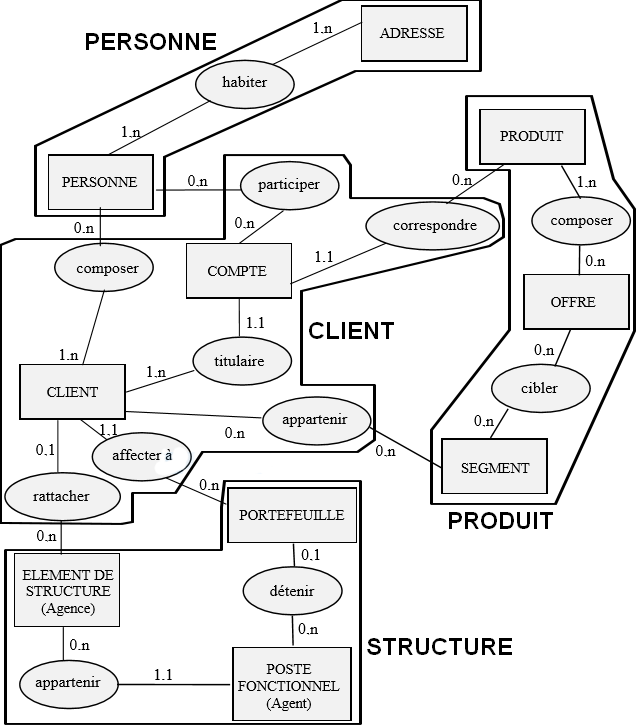
\includegraphics[width=\textwidth]{figures/mcd/MCD_Clients_Produits}
\caption{MCD Clients Produits}
\end{figure}


\subsection{Données commerciales}

\begin{figure}[H]
\centering
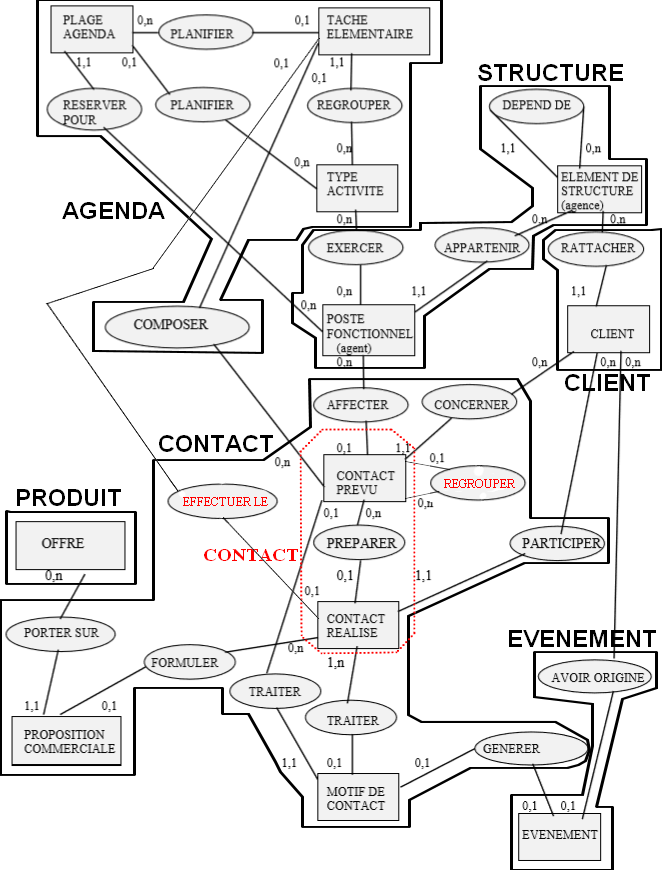
\includegraphics[width=\textwidth]{figures/mcd/MCD_Commercial}
\caption{MCD Commercial}
\end{figure}

\section{Diagramme d’état de l'objet métier \bf{contact}}

\begin{figure}[H]
\centering
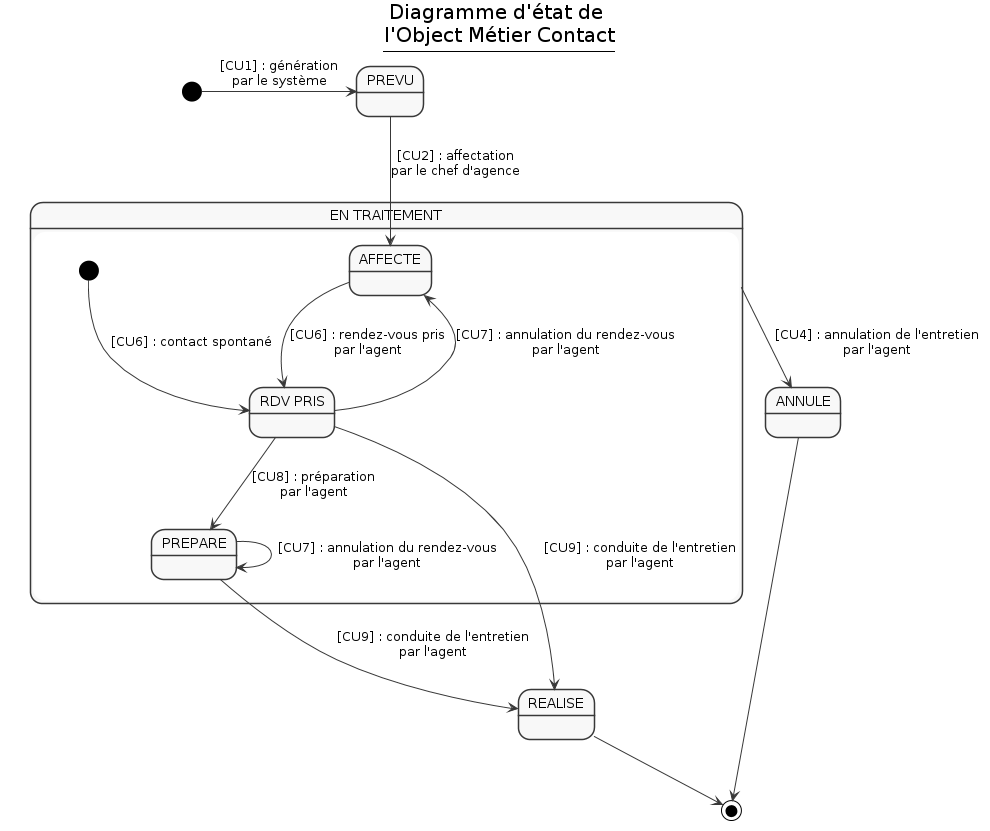
\includegraphics[width=\textwidth]{figures/diag_etats_contact}
\caption{Diagramme d'état de l'objet métier contact}
\end{figure}

\section{Architecture technique}

Cette section présente les choix techniques effectués dans le cadre de la conception de l'architecture technique.

\subsection{Choix du type d'IHM}

Nous avons choisi de concevoir un client léger sous forme d'une application web. Nous avons réalisé ce choix après considération de différents critères. Il nous semble plus facile de maintenir une application centralisée putôt qu'une application distribuée. En effet, dès qu'une mise à jour de l'application est réalisée, il est plus simple de mettre à jour l'application sur quelques serveurs que sur plusieurs centaines de postes clients. Cette application ne pouvant être utilisée hors ligne, un client lourd ne présente pas plus d'intérêt selon ce critère. Il est également important de prendre en compte le fait que le client lourd implique une grande quantité de travail pour l'adapter à des environnements différents tandis qu'un simple navigateur à jour permettra d'accèder à l'application. En effet, même si ce client lourd est développé dans un langage permettant la portabilité du code, il nécessitera l'installation de dépendances pour son fonctionnement ce qui n'est pas viable à long terme et implique des coûts importants en termes de ressources. 

\subsection{Serveurs et localisation}

La répartition des serveurs présentée dans la suite fait référence à la figure suivante présentant le diagramme d'organisation fourni dans le sujet.

\begin{figure}[H]
    \centering
	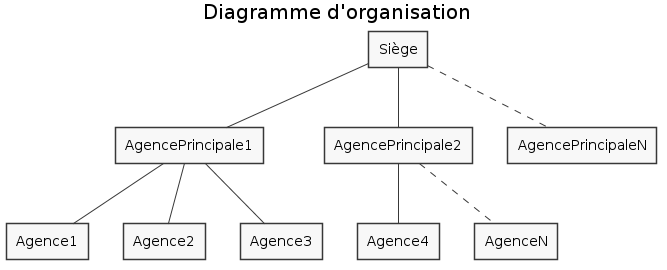
\includegraphics[scale=0.6]{figures/DO.png}
	\caption{Diagramme d'organisation}
\end{figure}

Nous avons répartis les serveurs de données en répondant aux questions suivantes :\\
\begin{itemize}
	\item[\textbullet] La donnée est-elle partagée ? Si oui, par qui ?
	\item[\textbullet] Quelle est la fréquence d'accès à la donnée ?
	\item[\textbullet] En terme de sécurité, qui a besoin d'accéder à la donnée ?\\
\end{itemize}

Nous avons donc abouti à une répartition optimale selon nos critères. Des serveurs de données seront implantés au siège (site central) ainsi que dans les agences principales mais pas dans les agences rattachées aux agences principales. \'Etant donné le fait que la gestion des données clients et produits est réalisée au siège, celui-ci nécessite évidemment des serveurs pour stocker ces données. Ensuite, il nous semble réaliste de distribuer la donnée propre à chaque agence au sein de l'angence principale à laquelle elle est rattachée. Cela permettra de ne pas surcharger d'information inutile les entités ne nécessitant pas l'accès à ces données. De plus, cela aura un effet important sur les performances globales du système et notamment la diminution du nombre de requêtes sur des sites distants qui aura pour effet de réduire les temps de réponse. Il nous semble par contre irréaliste de déployer un serveur de données par agence, ce qui entrainerait des coûts de maintenance non négligeables.\\

Nous avons procédé de la même manière concernant les serveurs d'applications en nous posant des questions différentes :\\
\begin{itemize}
	\item[\textbullet] Est-il possible et intéressant, étant donnée la répartition des serveurs de données, de distribuer les composants applicatifs ?
	\item[\textbullet] Quelles seraient les conséquences d'un tel déploiement ?\\
\end{itemize}

Nous sommes donc arrivés aux conclusions suivantes. Afin de profiter des avantages offerts par le client léger, nous ne devons pas trop répartir les serveurs d'applications et il n'est donc pas souhaitable d'équiper chaque agence d'un serveur d'applications. Il n'est pas non plus intéressant d'équiper seulement le siège d'un serveur d'application, en particulier si l'on considère la charge qu'il subira si toutes les agences font appel à ce serveur central. Il est également important de noter qu'en cas de dysfonctionnement du serveur d'application sur le site central, toutes les agences seront impactées. Il semble donc judicieux d'équiper chaque agence principale d'un serveur d'application. En effet, cela apporte de nombreux avantages. Parmis ceux-ci le fait de pouvoir déployer progressivement une nouvelle version d'un applicatif ce qui est pratiqué dans beaucoup de grands groupes avec des entités qui réalisent les tests des nouvelles versions sans impacter l'intégralité des agences jusqu'à la validation de la version. Cette répartition augmente également la tolérance aux pannes et réduit la charge réseaux induite par les postes clients. Un serveur d'applications devra tout de même être présent au siège pour supporter les composants applicatifs partagés.\\

Le tableau ci-dessous présente la synthèse de nos choix concernant la répartition des serveurs et le nombre de serveurs à implanter. Ces choix seront renforcés par les choix concernant la répartition des blocs applicatifs et les flux de données induits par cette architecture. 


\begin{table}[H]
    \centering
    \begin{tabular}{l|l|l}
    Type d'entité        & Serveur de Données & Serveur d'Applications \\ \hline
    Siège (site central) & Oui ($n$)            & Oui ($n$)                \\
    Agence principale    & Oui ($1$)            & Oui ($1$)                \\
    Agence simple        & Non                & Non                    \\
    \end{tabular}
    \caption{Tableau de répartition des serveurs par entité organisationnelle}
\end{table}

La figure suivante présente la répartition des serveurs.

\begin{figure}[H]
    \centering
    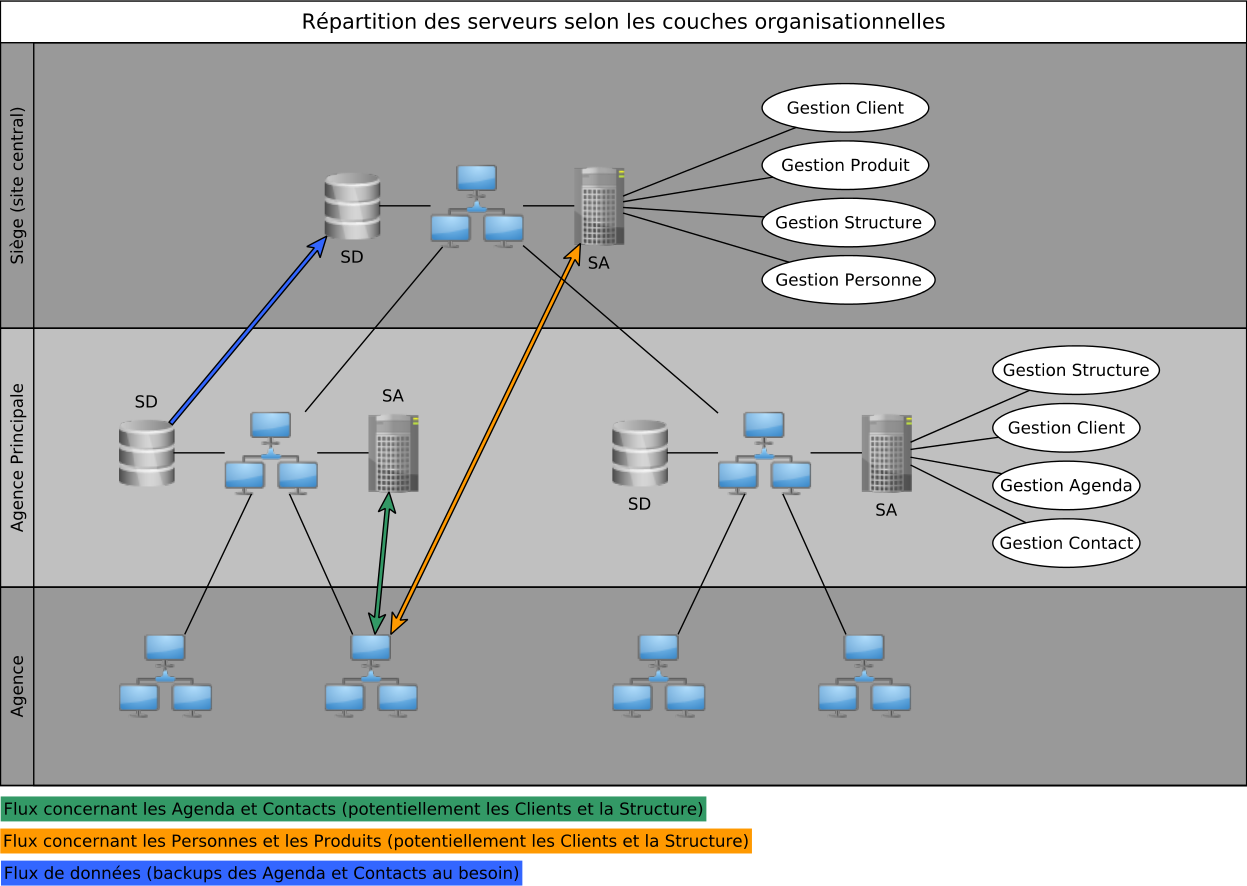
\includegraphics[scale=0.5]{figures/architectureServeurs.png}
    \caption{Plan de répartition des serveurs}
\end{figure}

\subsection{Implantation des composants du noyau applicatif et flux de données}

Etant donnée la répartition des serveurs précédemment exposée et la contrainte concernant la gestion des données client et produit nous avons jugé qu'il serait intéressant de déployer les blocs applicatifs Personne, Client, Produit et Structure sur le(s) serveur(s) d'applications situé(s) sur le site central. Il semble également envisageable de distribuer les composants Contact et Agenda sur les serveurs d'applications respectifs des différentes agences principales. Il pourrait être avantageux de répliquer les données concernant les clients et les structures au niveau des agences principales. \\

Si nous considérons les flux de données, relatifs à des opérations classiques, induits par ces différents choix nous obtenons les résultats suivants. Une opération de consultation ou d'édition de l'agenda ne ferait intervenir que les serveurs situés au niveau de l'agence. Seules les opérations liées aux clients ou aux produits feront intervenir les serveurs du site central. Enfin, la réplication des clients concernant une agence rattachée à une agence principale permettrait de gérer les évènements concernant les clients au niveau des agences principales également.
Du point de vue de la sécurité du système il est également intéressant de noter que la répartition choisie permet une bonne segmentation des données. Par exemple, la corruption d'un système au niveau d'une agence principale ne permettrait pas d'accèder aux agendas de toutes les agences ni à la liste de tous les clients. De même, les informations confidentielles concernant les clients seront toutes stockées au siège ce qui permettra une protection efficace de ces dernières. Dans le cas d'une corruption de ce système central, l'attaquant ne sera pas forcément en mesure de consulter les agendas des agences. Cette architecture nécessite par contre des protections adéquates des communications entre les différents systèmes distribués.
